\documentclass[11pt,a4paper]{article}
\usepackage{iftex}
\ifXeTeX
  \usepackage{fontspec}
  \setmainfont{Liberation Serif}
  \setsansfont{Liberation Sans}
  \setmonofont{Liberation Mono}
\else
  \usepackage[T2A]{fontenc}
  \usepackage[utf8]{inputenc}
\fi
\usepackage[russian]{babel}
\usepackage[margin=2cm]{geometry}
\usepackage{amsmath,booktabs,tabularx,array}
\usepackage{graphicx}
\usepackage[unicode,hidelinks]{hyperref}
\usepackage{xurl}
\setlength{\parindent}{1.25cm}
\setlength{\parskip}{3pt}
\renewcommand{\arraystretch}{1.15}
\title{Домашнее задание 5\\Факторная обеспеченность и торговля\\натуральным мёдом}
\author{10130}
\begin{document}
\maketitle
\noindent Товар исследования - натуральный мёд,  040900 HS6. Для сравнения используется HS2017 190590: прочие хлебобулочные изделия, рисовая бумага и аналогичные изделия. Основной источник торговли - OEC на данных CEPII BACI, база \texttt{trade\_i\_baci\_a\_17}. Период наблюдений -- 2018-2024 гг., сравнение рынков - 2021 и 2024 гг. Показатель фактора взят из World Bank WDI за 2024 г. Все результаты соответствуют расчётам в блокноте ДЗ-5. Денежные показатели приведены в текущих долларах США

\section*{Задание 1. Факторная гипотеза}

\subsection*{1а. Фактор и обеспеченность двух стран}
В 2024 г. пашня на человека составляла 0,846727 га в России и 0,032450 га в Японии. Отношение показателей равно
\[
\frac{f_{\mathrm{RUS}}}{f_{\mathrm{JPN}}}=26{,}093294
\]
По этому показателю обеспеченность России землёй примерно в 26,1 раза выше (Источник --- WDI, показатель \texttt{AG.LND.ARBL.HA.PC}, исходные сведения FAO )

Для меда выбрана земля: пчёлам нужны территории с цветущими растениями. По сравнению с производством готовых хлебобулочных изделий получение мёда предположительно сильнее зависит от местных природных условий и подходящих территорий. Поэтому рабочая гипотеза состоит в том, что мёд относительно землеёмок, а большая обеспеченность подходящей землёй может сопровождаться его чистым экспортом. При производстве хлебобулочных изделий земля также используется через выращивание сырья, поэтому противопоставление не является строгим

Это качественная оценка факторной ёмкости, а не измеренный коэффициент затрат земли на тонну меда. Сопоставимых данных о затратах земли и труда на единицу обоих товаров в расчётах нет. Пашня на человека характеризует страну, а не технологию товара. Кроме того, пчеловодство возможно на лесных и других территориях, которые показатель пашни не охватывает [2]. Поэтому выбранное приближение имеет заметные ограничения.

\begin{center}
\begin{tabular}{lrr}
\toprule
Страна & Пашня, га/чел. & Год\\
\midrule
Россия & 0,846727 & 2024\\
Япония & 0,032450 & 2024\\
\bottomrule
\end{tabular}
\end{center}

\subsection*{1б. Порядок по фактору и относительному экспорту}
В 2024 г. российский экспорт меда составил 7\,314\,791 долл., а товара сравнения  215\,060\,721 долл. В Японии соответствующие значения равны 578\,331 и 332\,821\,322 долл.
\[
RX_i=\frac{X_{i,p}}{X_{i,q}}.
\]
\begin{center}
\begin{tabular}{lrrr}
\toprule
Страна & Экспорт мёда, долл. & Экспорт HS 190590, долл. & $RX$\\
\midrule
Россия & 7\,314\,791 & 215\,060\,721 & 0,034013\\
Япония & 578\,331 & 332\,821\,322 & 0,001738\\
\bottomrule
\end{tabular}
\end{center}
Экспорт меда составляет около 3,40\% от экспорта товара сравнения в России и 0,17\% в Японии. Это отношение двух потоков, а не доля меда во всём экспорте страны. В России выше и обеспеченность землёй, и $RX$. Такой порядок согласуется с рабочей факторной гипотезой и логикой теоремы Хекшера--Олина, если предположение о большей землеёмкости мёда верно. Сам по себе расчёт это предположение не доказывает.

\subsection*{1в. Устойчивость по годам}
Во всех 7 годах, с 2018 по 2024 г., российский $RX$ был выше японского. Следовательно, порядок не зависит только от результата 2024 г. При этом устойчивое совпадение не доказывает теорему. Во-первых, технологии и качество факторов в странах могут различаться. Во-вторых, на экспорт влияют внутренний спрос, торговые барьеры и стоимость доставки. Кроме того, обеспеченность землёй здесь сравнивается за 2024 г., а не отдельно за каждый год ряда.

\begin{center}
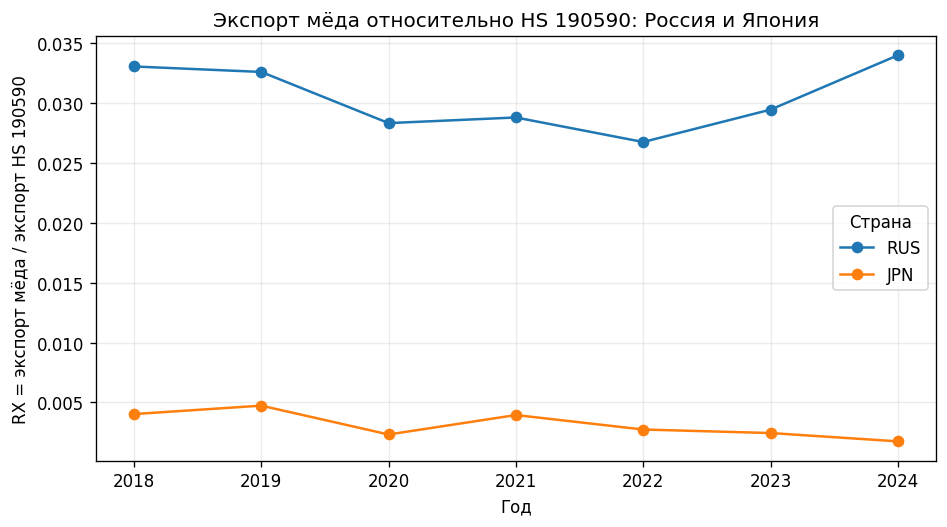
\includegraphics[width=.9\linewidth]{figures/rx_years.png}
\end{center}
\noindent Источник графика: расчёты пункта 1в блокнота, OEC / BACI [3].

\section*{Задание 2. Выборка стран}

\subsection*{2а. Нормированный чистый экспорт}
В России в 2024 г. экспорт натурального мёда равен 7\,314\,791 долл., импорт --- 108\,806 долл., а $NEX=0{,}970686$. Показатель рассчитан как
\[
NEX_i=\frac{X_i-M_i}{X_i+M_i}.
\]
Положительное значение означает преобладание экспорта. Показатель находится от $-1$ до $1$ при положительном обороте: $-1$ соответствует только импорту, $1$ --- только экспорту, а ноль --- равным потокам. Он не измеряет выпуск или внутреннее потребление. В выборке 16 стран, товар --- HS2017 040900, торговля --- OEC / BACI, фактор --- пашня на человека из WDI. Оба набора относятся к 2024 г. Если рабочая гипотеза верна, страны с большей обеспеченностью землёй должны чаще иметь положительный $NEX$ мёда.

\subsection*{2б. Диаграмма и исключения}
Самые высокие значения фактора в выборке имеют Австралия (1,149690 га/чел.), Аргентина (1,025074), Канада (0,922488) и Россия (0,846727). У Австралии, Аргентины и России $NEX$ положителен, у Канады --- немного отрицателен. Низкие значения имеют Южная Корея (0,025159) и Япония (0,032450), обе страны являются чистыми импортёрами. При разделении по медиане 0,130689 га/чел. С ожиданием согласуются Южная Корея, Япония, Нидерланды, Ирландия, Великобритания, Саудовская Аравия, Бразилия, Россия, Аргентина и Австралия. Не согласуются Китай, Новая Зеландия, Германия, Франция, США и Канада. Два заметных исключения --- США и Новая Зеландия: у США фактор выше медианы, но $NEX=-0{,}937224$; у Новой Зеландии ниже медианы, но $NEX=0{,}998796$. На диаграмме видны оба типа наблюдений, поэтому одного показателя земли недостаточно для объяснения торговли.

\begin{center}
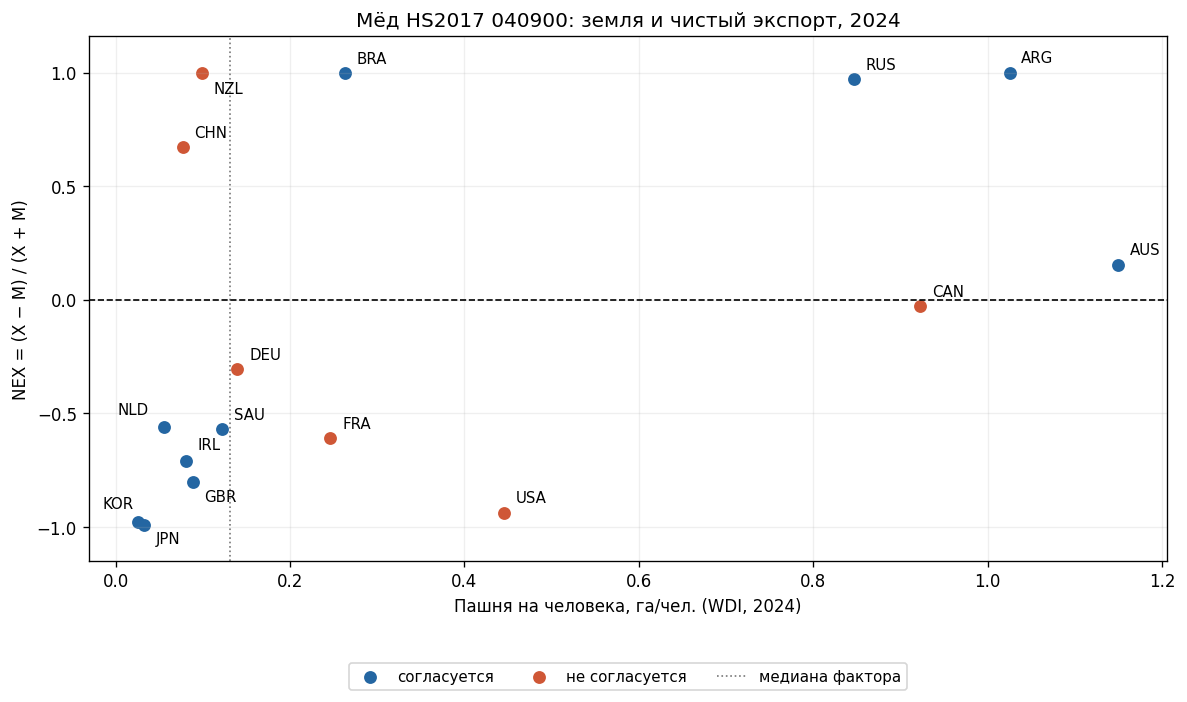
\includegraphics[width=\linewidth]{figures/nex_scatter.png}
\end{center}
\noindent Синие точки --- страны, согласующиеся с ожиданием, красные --- исключения. Пунктир по вертикали --- медиана фактора. Источник: пункт 2б блокнота, OEC / BACI и WDI.

\subsection*{2в. Результат по группам}
Доля чистых экспортёров в группе с высоким фактором равна 50\%, а с низким --- 25\%. В каждой группе по 8 стран; чистых экспортёров соответственно 4 и 2. Порядок долей поддерживает простое факторное ожидание в этой выборке, но не является строгим доказательством. Исключения есть с обеих сторон: Китай и Новая Зеландия экспортируют больше, чем импортируют, при низком показателе пашни, а США, Германия, Франция и Канада имеют высокий показатель и отрицательный $NEX$. Это требует дополнительного объяснения, а не автоматического признания данных ошибочными.

\subsection*{2г. Проверка торгового оборота}
Медиана оборота составляет 117\,006\,248,50 долл. После отбора стран с оборотом не ниже медианы сохраняются исключения Китай, Новая Зеландия, Германия, Франция и США; Канада отсеивается. Например, у Новой Зеландии оборот равен 251\,461\,006 долл., поэтому её результат не связан с совсем маленькими потоками. Первое возможное объяснение --- пашня плохо отражает подходящие для пчеловодства природные условия. Это можно проверить по площади и составу медоносных территорий, используя сведения FAO и статистику землепользования Новой Зеландии. Второе объяснение --- различия технологий и качества продукции. Для проверки нужны данные о выходе мёда на пчелиную семью из FAOSTAT или национальной статистики, а также стоимости и количестве экспорта из OEC. Эти объяснения пока являются гипотезами. Результат не является буквальным парадоксом Леонтьева: факторное содержание экспортной и импортной корзин не рассчитано.

\section*{Задание 3. Гипотезы о зарубежных рынках}

\subsection*{3а. Сопоставление шести рынков}
В 2024 г. импорт Японии составил 0,132238 млрд долл., а Южной Кореи --- 0,016457 млрд долл. У Японии более отрицательный $NEX$ ($-0{,}991291$ против $-0{,}976061$), но с 2021 г. стоимость её импорта сократилась на 21,576202\%, тогда как в Корее выросла на 9,440330\%. Пашня на человека в обеих странах невелика: 0,032450 и 0,025159 га соответственно. Всего выбраны шесть рынков: США и Германия как два крупнейших импортёра базы, Нидерланды и Ирландия как страны с ростом импорта, а также Япония и Южная Корея из предыдущего исследования. Размер импорта показывает денежный масштаб потока, рост --- его изменение за период, а $NEX$ --- соотношение экспорта и импорта. Эти показатели нельзя подменять друг другом.

\begin{center}
\small
\begin{tabular}{lrrrrr}
\toprule
Страна & Импорт 2021 & Импорт 2024 & Изменение, \% & $NEX$ & Фактор\\
\midrule
США & 0,626533 & 0,621239 & $-0,844842$ & $-0,937224$ & 0,445740\\
Германия & 0,337941 & 0,248965 & $-26,328754$ & $-0,304280$ & 0,139565\\
Нидерланды & 0,067406 & 0,074510 & 10,539382 & $-0,561867$ & 0,055742\\
Ирландия & 0,017688 & 0,024809 & 40,263313 & $-0,709784$ & 0,080248\\
Япония & 0,168619 & 0,132238 & $-21,576202$ & $-0,991291$ & 0,032450\\
Южная Корея & 0,015037 & 0,016457 & 9,440330 & $-0,976061$ & 0,025159\\
\bottomrule
\end{tabular}
\end{center}
\noindent Импорт --- млрд долл. США; фактор --- га пашни на человека, 2024 г. Источники: пункты 3а и 3б блокнота, OEC / BACI и WDI.

\subsection*{3б. Три проверяемые гипотезы}
Среди шести стран Япония занимает первое место по более отрицательному $NEX$, Ирландия --- по росту импорта, США --- по его размеру. Гипотеза 1: при прочих равных дефицит подходящей земли усиливает чистый импорт мёда; низкие значения фактора Японии и Кореи согласуются с этим ожиданием. Ей противоречило бы устойчивое преобладание экспорта у стран с малой обеспеченностью именно подходящей землёй при сопоставимых технологиях и спросе. Проверять нужно качество и состав земель, а не только пашню. Гипотеза 2: первое место Ирландии по росту может быть связано с расширением внутреннего спроса. Для проверки нужны физические объёмы импорта, внутренний выпуск и потребление; гипотеза не подтвердится, если рост стоимости объясняется только ценами или последующим реэкспортом. Гипотеза 3: Германия занимает второе место по импорту, но последнее из шести по более отрицательному $NEX$, потому что относительно много экспортирует. Возможное объяснение --- переработка и доступ к соседним рынкам, снижающий торговые издержки. Нужны данные о направлениях экспорта, происхождении товара и перевозке; объяснение не подтвердится, если встречные потоки не связаны с такой деятельностью. Места не складываются в общий рейтинг.

\subsection*{3в. Южная Корея и Япония}
Разности «Южная Корея минус Япония» равны $-0{,}115781$ млрд долл. по импорту 2024 г., $+31{,}016532$ процентного пункта по его изменению и $+0{,}015230$ по $NEX$. Корея меньше по масштабу, но имеет положительную динамику. Цепочка для Кореи: рост стоимости импорта --- возможное расширение спроса --- проверка количества, цен и внутреннего потребления. Япония существенно больше по импорту и имеет более отрицательный $NEX$, но её импорт сократился. Цепочка для Японии: большой поток при снижении стоимости --- возможное изменение цен или внутреннего спроса --- проверка физических объёмов, выпуска и цен по видам мёда. Ограничения анализа: HS6 объединяет разное качество мёда; стоимость не равна количеству; пашня не измеряет площадь медоносов; технологии стран не одинаковы, хотя классическая модель это предполагает; не учтены внутренний спрос, тарифы, санитарные требования и доставка. Поэтому расчёты дают основания для дальнейшего сравнения, но не для окончательного выбора рынка.

\subsection*{3г. Публикации к выводам}
В расчётах фактор измерен в гектарах пашни на человека. Описание WDI [1] подтверждает единицы и определение, но не показывает затраты земли на производство мёда. Публикация FAO [2] поясняет, что пчеловодство связано с цветущими растениями и возможно на разных территориях. Она поддерживает ограничение выбранного показателя, но не доказывает, что мёд землеёмче товара сравнения. Метаданные OEC [3] подтверждают HS2017 и доллары США для \texttt{Trade Value}, но не позволяют считать рост стоимости ростом количества. Поэтому источники уточняют границы выводов, а не заменяют их проверку.

\section*{Источники}
\begin{enumerate}
\item World Bank / FAO. \textit{WDI Metadata Glossary: Arable land (hectares per person), AG.LND.ARBL.HA.PC}. Дата публикации страницы не указана.\\
\url{https://databank.worldbank.org/metadataglossary/world-development-indicators/series/AG.LND.ARBL.HA.PC}\\
Данные: \url{https://api.worldbank.org/v2/country/all/indicator/AG.LND.ARBL.HA.PC?format=json&date=2020:2024&per_page=20000}
\item Bradbear N. / FAO. \textit{Beekeeping and sustainable livelihoods}. FAO Diversification booklet 1, 2004. Раздел о ресурсах пчеловодства.\\
\url{https://www.fao.org/4/y5110e/y5110e02.htm}
\item OEC / CEPII BACI. \textit{HS6 REV. 2017 (2018--2024)}, база \texttt{trade\_i\_baci\_a\_17}. Дата публикации метаданных не указана.\\
\url{https://api.oec.world/tesseract/cubes/trade_i_baci_a_17}\\
Данные: \url{https://api.oec.world/tesseract/data.jsonrecords}; товары: HS6 1040900 и 4190590 в идентификаторах OEC, потоки экспорта и импорта по годам и странам. Полные ссылки запросов приведены в журнале источников блокнота.
\end{enumerate}

\end{document}
